\chapter{Aspectos Conceituais}

\section{Inteligência Artificial}

%Um pouco de história, referências básicas sobre o assunto, usos mais
%comuns, estado da arte.

A Inteligência Artificial (IA) é uma área de pesquisa da Ciência da Computação e da Engenharia da Computação, dedicada a buscar métodos ou dispositivos computacionais que possuam ou simulem a capacidade racional de resolver problemas, pensar ou, de forma ampla, ser inteligente.

Apenas recentemente, com o surgimento do computador moderno, é que a inteligência artificial ganhou meios e massa crítica para se estabelecer como ciência integral, com problemáticas e metodologias próprias. Desde então, seu desenvolvimento tem extrapolado os clássicos programas de xadrez ou de conversão e envolvido áreas como visão computacional, análise e síntese da voz, lógica difusa, redes neurais artificiais e muitas outras.
Inicialmente a IA visava reproduzir o pensamento humano. A Inteligência Artificial abraçou a idéia de reproduzir faculdades humanas como criatividade, auto-aperfeiçoamento e uso da linguagem. Porém, o conceito de inteligência artificial é bastante difícil de se definir. Por essa razão, Inteligência Artificial foi (e continua sendo) uma noção que dispõe de múltiplas interpretações, não raro conflitantes ou circulares.

\subsection{História}

O primeiro trabalho a respeito de IA foi realizado por Warren McCulloch e Walter Pitts em 1943, em que demonstrava um modelo de neurônios artificiais, em que cada neurônio poderia estar ``ligado'' ou ``desligado'', isso dependeria dos estados em que os neurônios vizinhos estariam~\cite{livro_russel}.

Donald Hebb demonstrou em 1949 uma regra de atualização simples para definir a intensidade de conexão entre neurônios, essa regra é influente ainda nos dias de hoje~\cite{livro_russel}.

Em 1950 Alan Turing publicou o artigo \textit{``Computing Machinery and Intelligency''}~\cite{artigo_turing}. Neste artigo ele apresentou diversos algoritmos de IA e seu famoso teste, o ``Teste de Turing''~\cite{livro_russel}.

Em 1951, no departamento de matemática de Princeton, Marvin Minsk e Dean Edmound apresentaram o primeiro computador de rede
neural, o SNARC era composto por 3000 válvulas e simulava uma rede de 40 neurônios~\cite{livro_russel}.

Segundo Stuart Russel~\cite{livro_russel}, cinco anos após o SNARC John McCarthy realizou um seminário em Dartmouth, reunindo todos os grandes pesquisadores do conhecimento. Nesse seminário Allen Newell e Herbert Simon do Carnegie Tech apresentaram o \textit{Logic Theorist} o primeiro programa de raciocínio. Nesse seminário John McCarthy juntamente com os outros seminaristas percebeu que a IA devia ser um campo separado, e não uma ramificação da matemática nem mesmo estar sob o nome de pesquisa operacional ou teoria de controle, então eles definiram o nome de Inteligência Artificial e, após este seminário a IA foi definida como o campo em que tenta construir máquinas que funcionem de forma autônoma e em ambientes mutáveis.


Pesquisas sobre inteligência artificial foram intensamente custeadas na década de 1980 pela Agência de Projetos de Pesquisas Avançadas sobre Defesa (\textit{“Defense Advanced Research Projects Agency”}), nos Estados Unidos, e pelo Projeto da Quinta Geração (\textit{“Fifth Generation Project”}), no Japão. O trabalho subsidiado fracassou no sentido de produzir resultados imediatos, a despeito das promessas grandiosas de alguns praticantes de IA, o que levou proporcionalmente a grandes cortes de verbas de agências governamentais no final dos anos 80, fase conhecida como \emph{o inverno da IA}. No decorrer da década seguinte, muitos pesquisadores de IA mudaram para áreas relacionadas com metas mais modestas, tais como aprendizado de máquinas, robótica e visão computacional, muito embora pesquisas sobre IA pura continuaram em níveis reduzidos.

Os fatos acima listados marcam o nascimento e desenvolvimento da inteligência artificial, daquela época até os dias de hoje ocorreram grandes avanços neste ramo da computaçao. 

Atualmente a IA está mais madura e não possui mais aquele ar de pioneirismo do inicio. O pesquisador de IA deve provar suas teorias com diversos experimentos empíricos e a demonstração dos resultados, e com o surgimento da Internet os pesquisadores foram capazes de compartilhar as evoluções de suas pesquisas e acelerar os processos de desenvolvimento.

Encorajados pela resolução dos subproblemas da IA, os pesquisadores começaram a examinar o problema do ``agente como um todo''. O movimento estabelecido tem como objetivo entender o funcionamento interno de agentes incorporados a ambientes reais com entradas sensoriais continuas. Um dos ambientes mais importantes para os agentes inteligentes é a Internet, diversas ferramentas utilizam a Inteligência Artificial na Internet, tais como mecanismos de pesquisas, sistemas de recomendação e sistemas de construção de web sites.~\cite{livro_russel}
Na tentativa de se construir agentes percebeu-se que subcampos que anteriormente eram isolados da IA, precisavam de uma reorganização para o melhor aproveitamento de seus resultados.
Outra conseqüência foi que a IA se aproximou de outras áreas, como a teoria de controle e a economia, áreas que também lidam com agentes.~\cite{livro_russel}
No século XXI há um grande interesse em \textit{Agentes Inteligentes} uma nova ramificação que pretende reunir todas as subáreas da IA, pois se percebeu que todas juntas poderiam criar um Agente perfeito realizando o principal objetivo da IA, entender o pensamento humano.

Entre os teóricos que estudam o que é possível fazer com a IA existe uma discussão onde se consideram duas propostas básicas: uma conhecida como ``forte'' e outra conhecida como ``fraca''.
A grosso modo podemos diferenciar as duas propostas da seguinte forma:
\begin{itemize}
\item IA Fraca: As máquinas podem simular um comportamento inteligente, agir como se fossem inteligentes.
\item IA Forte: As máquinas podem realmente pensar e não apenas simular o pensamento.
\end{itemize}

\subsection{Áreas de aplicação}
Enquanto que o progresso direcionado ao objetivo final de uma inteligência similar à humana tem sido lento, muitas derivações surgiram no processo. Exemplos notáveis incluem as linguagens LISP e Prolog, as quais foram desenvolvidas para pesquisa em IA, mas agora possuem funções não-IA. A cultura Hacker surgiu primeiramente em laboratórios de IA, em particular no MIT AI Lab, lar de celebridades tais como McCarthy, Minsky, Seymour Papert (que desenvolveu a linguagem Logo), Terry Winograd (que abandonou IA depois de desenvolver SHRDLU).
Muitos outros sistemas úteis têm sido construídos usando tecnologias que ao menos uma vez eram áreas ativas em pesquisa de IA. Alguns exemplos incluem:~\cite{kishimoto}
\begin{itemize}
\item Planejamento automatizado e escalonamento: a uma centena de milhões de quilô\-metros da Terra, o programa Remote Agent da NASA se tornou o primeiro programa de planejamento automatizado (autônomo) de bordo a controlar o escalonamento de operações de uma nave espacial.
\item Jogos: O Deep Blue da IBM se tornou o primeiro programa de computador a derrotar o campeão mundial em uma partida de xadrez, ao vencer Garry Kasparov.
\item Controle autônomo: O sistema de visão de computador ALVINN foi treinado para dirigir um automóvel, mantendo-o na pista.
\item Robótica: Muitos cirurgiões agora utilizam robôs assistentes em microcirurgias.
\item Lógica incerta: Técnica para raciocinar dentro de incertezas, tem sido amplamento usada em sistemas de controles industriais.
\item Redes Neurais: Vêm sendo usadas em uma larga variedade de tarefas, desde sistemas de detecção de intrusos a jogos de computadores.
\item Aplicações utilizando Vida Artificial são utilizados na indústria de entretenimento e no desenvolvimento da Computação Gráfica.
\item Sistemas baseados na idéia de agentes artificiais, denominados Sistemas Multiagentes, têm se tornado comuns para a resolução de problemas complexos.
\end{itemize}
Atualmente existem muitas aplicações práticas que envolvem conceitos de inteligência artificial. Dentre todas as áreas que, de alguma forma implementam conceitos de IA, os jogos eletrônicos tem ganhado grande destaque nos últimos anos.

\section{Jogos digitais}


Atualmente um dos maiores desafios para os desenvolvedores de jogos é a criação de um jogo com um bom desafio para o jogador, já que os jogos estão num nível gráfico e sonoro próximo da realidade. Diversos algoritmos já estão sendo usados pelas produtoras de jogos para a simulação de uma inteligência humana convincente. Houve uma preocupação enorme por parte das empresas desenvolvedoras de jogos em acompanhar a evolução tecnológica dos últimos tempos, com isso nasceram novos consoles poderosos como o Xbox da Microsoft, o Playstation 3 da Sony e o Nintendo Wii, porém, pouco foi feito com relação ao conteúdo dos jogos. É muito fácil observar este fenômeno, basta notar que atualmente os jogos que mais são lançados são continuações de jogos antigos com gráficos mais bonitos.
Os jogos que mais provam esta teoria são os RPGs (Role-Playing Game) e os jogos de aventura onde o jogador controla um personagem dentro de um universo e  interage com outros jogadores ou \npc{}s. Apesar de toda qualidade gráfica oferecida por estes jogos, todos possuem uma lógica parecida, o usuário deverá realizar as mesmas tarefas para completar o jogo, no melhor caso existe mais de uma maneira de realizar uma mesma tarefa, no entanto, o jogo será sempre o mesmo, os \npc{}s sempre dirão as mesmas falas e farão as mesmas coisas não importa quantas vezes o usuário jogue.
Um jogo que representa bem este fato é o jogo da Nintendo ``Legend of Zelda: Ocarina of Time'', nele o jogador controla um personagem que vive uma aventura para salvar uma princesa, na época em que foi lançado e até hoje o jogo ainda é um grande sucesso da Nintendo, no entanto, não importa quantas vezes seja jogado, a história é sempre a mesma, os diálogos com os \npc{}s são sempre os mesmos diálogos limitados, os poucos momentos em que o jogador pode ``falar'' com um \npc{} é para dizer ``sim'' ou ``não'' (figura \ref{zelda}) e em alguns casos é obrigado a escolher uma resposta pois a outra faz com que o \npc{} apenas repita a pergunta! Isso prejudica o jogo, pois uma vez que o usuário o termina, não existe mais a sensação do desafio a ser superado se ele jogar novamente, ou seja, a diversão associada ao jogo diminui.
Talvez com um pouco de esforço e dedicação seja possível desenvolver jogos que não sejam tão simples e superficiais, onde os \npc{}s tenham ``vontades'' e possam dialogar com o usuário de forma mais parecida com a realidade humana. Outro ponto interessante seria se o \npc{} mudasse seu perfil toda vez que o jogador recomeçasse o jogo, tornando-o mais imprevisível.

\begin{figure}
\centering
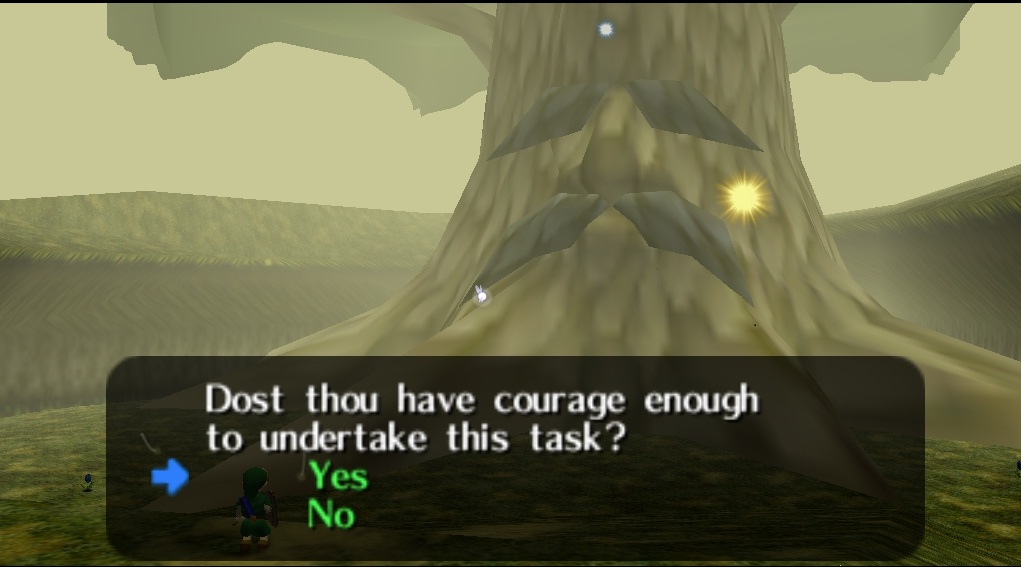
\includegraphics [width=\textwidth]{figuras/exemplo_dialogo_zelda.jpg}
\caption{Diálogo onde o jogador participa em Zelda Ocarina of Time}
\label{zelda}
\end{figure}


%Uma curta evolução histórica, tendências atuais (puxando um pouco para os problemas de IA --- a questão da imprevisibilidade e adaptabilidade dos jogos). Referências.

\section{Inteligência em jogos}

O principal objetivo do uso de técnicas de inteligência artificial em jogos eletrônicos é a diversão. Por causa disso, o conceito de IA acabou recebendo outra interpretação por parte dos desenvolvedores de jogos, surgiu o conceito de \textit{Game AI}.

Diferentemente da IA acadêmica que busca solucionar problemas extramamente difíceis, como imitar o reconhecimento que os humanos são capazes de realizar (reconhecimento facial e de imagens e objetos, por exemplo), ou mesmo entender e construir agentes inteligentes, a IA para jogos se preocupa com os resultados que o sistema irá gerar, e não como o sistema chega até os resultados. Isso se deve ao fato que jogos eletrônicos são negócios, e seus consumidores os compram em busca de diversão, e não lhes interessa como a inteligência de um personagem no jogo foi criada, desde que ela transforme o jogo divertido e desafiador, além, claro, de tomar decisões coerentes com o contexto do jogo.

Um exemplo que deixa claro a utilidade da IA para jogos são os \textit{shooters}. Nos jogos de tiros existem várias técnicas de IA que podem ser aplicadas. Por exemplo, é possível fazer com que os \npc{}s se comuniquem e criem estratégias para tentar cercar um inimigo, fato que pode tornar o jogo ainda mais interessante, no entanto, também é possível utilizar técnicas de IA para fazer com que os \npc{}s acertem todos os disparos na cabeça de seus inimigos, fato que passa longe da realidade humana, e que poderia prejudicar a qualidade do jogo do ponto de vista de um usuário.

No começo do desenvolvimento de jogos eletrônicos, a programação de IA era mais usualmente conhecida por \textit{programação de jogabilidade}, pois não havia nada de inteligente sobre os comportamentos exibidos pelos personagens controlados pelo computador. 
A figura \ref{IA em jogos} contém alguns exemplos de como a IA foi utilizada em jogos com o passar do tempo.

\begin{figure}
\centering
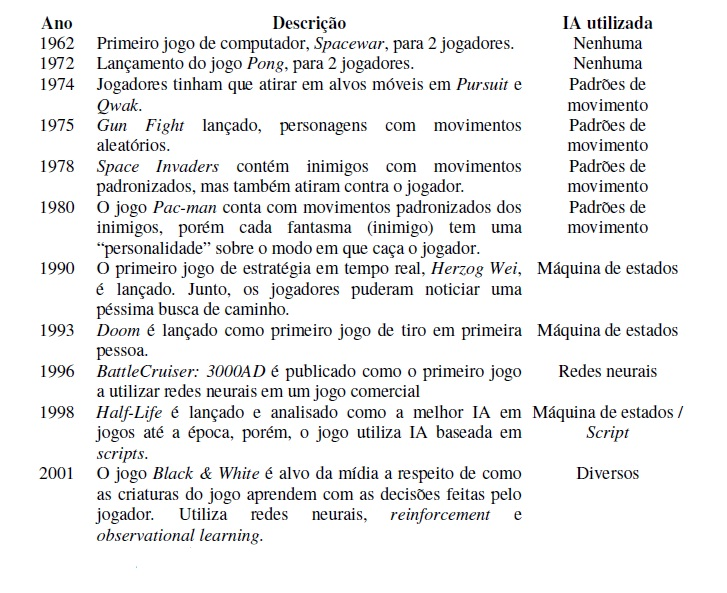
\includegraphics [height=10cm]{figuras/evolucao_IA_jogos.jpg}
\caption{Evolução da aplicação de IA em jogos~\cite{brian_schwab}}
\label{IA em jogos}
\end{figure}


\subsection{Crença, desejo e intenção --- a arquitetura BDI}

O modelo BDI (\textit{Beliefs Desires Intentions}) foi originalmente proposto por Bratman como uma teoria filosófica do raciocínio prático, propondo uma análise do comportamento humano que seria baseado em crenças, desejos e intenções.
Basicamente supõe-se que as ações são derivadas a partir de um processo chamado raciocínio prático. Este processo é constituído por duas etapas, na primeira, deliberação, o agente seleciona um conjunto de desejos que devem ser alcançados, de acordo com a situação atual das crenças do mesmo. Na segunda etapa ocorre a determinação de como os desejos produzidos no passo anterior podem ser atingidos através do uso dos meios disponíveis ao agente~\cite{wooldrige_agentes}

A seguir explicaremos melhor o que são crenças, desejos e intenções.
\begin{itemize}
\item \textbf{Crenças (Beliefs)}: Representam as características do ambiente e são atualizadas constantemente. Podem ser vistas como a componente informativa do sistema.
\item \textbf{Desejos (Desires)}: Representam os objetivos a serem alcançados. Podem ser vistos como motivações do sistema.
\item \textbf{Intenções (Intentions)}: Representam o atual plano de ações escolhido. 
\end{itemize}

A partir deste modelo nasceu a arquitetura BDI para agentes. Agentes BDI são sistemas localizados em um ambiente (em nosso caso o ambiente será virtual) sujeito a variações, além disso, percebem o estado deste ambiente constantemente e podem atuar sobre o mesmo para tentar alterar o estado atual.
Abaixo vemos o processo de raciocínio prático de um agente BDI.
 
\begin{figure}
\centering
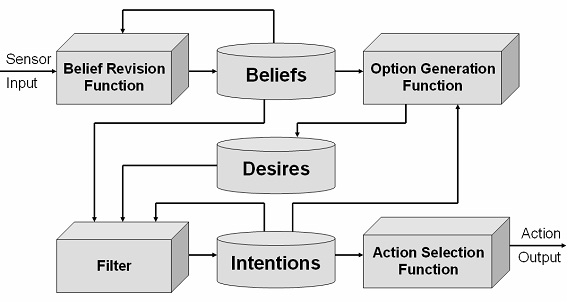
\includegraphics{figuras/visao_BDI.jpg}
\caption{Diagrama de uma arquitetura BDI genérica~\cite{wooldrige_agentes}}
\label{arquitetura BDI}
\end{figure}

Como se pode observar na figura \ref{arquitetura BDI}, existem sete elementos básicos que compõem um agente BDI, são eles~\cite{oliveira_BDI}:

\begin{itemize}
\item Um conjunto de crenças (\textit{Desires}) atuais que representam as informações que o agente tem do ambiente.
\item Uma função de revisão de crenças (\textit{Belief Revision Function}), a qual determina um novo conjunto de crenças a partir da percepção da entrada e das crenças do agente.
\item Uma função de geração de opções (\textit{Option Generation Function}), a qual determina as opções disponíveis ao agente (seus desejos), com base nas suas crenças sobre seu ambiente e nas suas intenções.
\item Um conjunto de opções (\textit{desires}) corrente que representa os possíveis planos de ações disponíveis ao agente.
\item Uma função de filtro (\textit{filter}), a qual representa o processo de deliberação do agente, que determina as intenções do agente com base nas suas crenças, desejos e inten\-ções atuais.
\item Um conjunto de intenções (\textit{Intentions}) atual, que representa o foco atual do agente, isto é, aqueles estados que o agente está determinado a alcançar.
\item Uma função de seleção de ação (\textit{Action Selection Function}), a qual determina uma ação a ser executada com base nas suas intenções atuais.
\end{itemize}

\subsection{Quadro-negro --- blackboard}

	A forma mais simples de apresentar o conceito de blackboard é através de uma metáfora que propõem a seguinte situação  “Imagine um grupo de cientistas reunidos em uma sala trabalhando de forma cooperativa para resolver um problema. Para chegar a uma solução é utilizado um quadro negro (\textit{blackboard}).
A resolução do problema começa quando o mesmo é escrito no quadro negro juntamente com informações iniciais. Os cientistas verificam o conteúdo do quadro e aguardam uma oportunidade para aplicar seus conhecimentos visando solucionar o problema. Quando um cientista encontra informações suficientes para fazer uma contribuição, o mesmo coloca sua contribuição no quadro negro, e com sorte, este processo ativará outro cientista e assim por diante até chegarem à solução do problema.”
	Dessa metáfora se pode concluir que um blackboard possui uma base de dados comum a diversos sistemas que estão tentando solucionar um problema e utilizam e atualizam as informações existentes nesta base de dados.
	 A seguir apresentaremos algumas características desta técnica:
	 \begin{itemize}
	 \item \textbf{Independência de conhecimento}: No exemplo acima, supomos que cada cientista adquiriu seus conhecimentos de maneira independente dos outros, ou seja, num blackboard cada sistema que participa da solução de um problema tem seus próprios níveis de conhecimento, independentemente dos outros sistemas.
	 \item \textbf{Diversidade nas técnicas de solução de problemas}: Uma das grandes vantagens do blackboard é que não interessa como os sistemas que estão trabalhando na resolução do problema funcionam, ou seja, um sistema pode utilizar redes neurais enquanto outro pode utilizar outra técnica, que para o blackboard estas “fontes de conhecimento” são caixas pretas que fazem suas contribuições.
	 \item \textbf{Representação da informação é flexível}: Não existe nenhuma definição de como deve ser a informação, dando liberdade a quem implementa de definir como representar os dados.
	 \item \textbf{Linguagem comum entre os sistemas}: Ao mesmo tempo em que existe a flexibilidade na representação da informação, é necessário, por outro lado, que todos os sistemas envolvidos sejam capazes de entender tais informações.
	 \item \textbf{Liberdade de organização dos dados}: A organização dos dados é livre, porém, deve ser feita de tal forma que, no caso da base de dados possuir muita informação, seja fácil para um sistema encontrar informações específicas de forma rápida e simples.
	 \item \textbf{Ativações baseadas em eventos}: Os sistemas que estão trabalhando na solução do problema não se comunicam diretamente, ao invés disto, todos “observam” a base de dados comum e utilizando as informações da mesma buscam gerar novos dados que são colocados na mesma base, tais dados podem ativar outro sistema que fará a mesma coisa até que o problema seja completamente resolvido.
	 \item \textbf{Necessidade de controle}: É preciso haver um “órgão” para controlar todos os sistemas e decidir quem deve e quem não deve poder alterar os dados do quadro negro, assim não existe o risco de mais de um sistema alterar uma mesma área de dados simultaneamente.
	 \item \textbf{Geração de solução incremental}: É evidente que a solução de um problema acontece de passo em passo, ou seja, um sistema faz uma contribuição com novos dados, a seguir, outro sistema utiliza tais dados e faz uma nova contribuição e de ciclo em ciclo o problema tende a ser resolvido. 
	 \end{itemize}

Na figura \ref{blackboard} temos uma visão geral de como funciona o blackboard. Basicamente existem fontes de conhecimento (sistemas que estão trabalhando na resolução do problema) um sistema de controle que concede permissões às fontes de conhecimento para alterarem os dados do quadro negro, este por sua vez, é uma base de dados que contem informações que ficam disponíveis a todas as fontes de conhecimento.

\begin{figure}
\centering
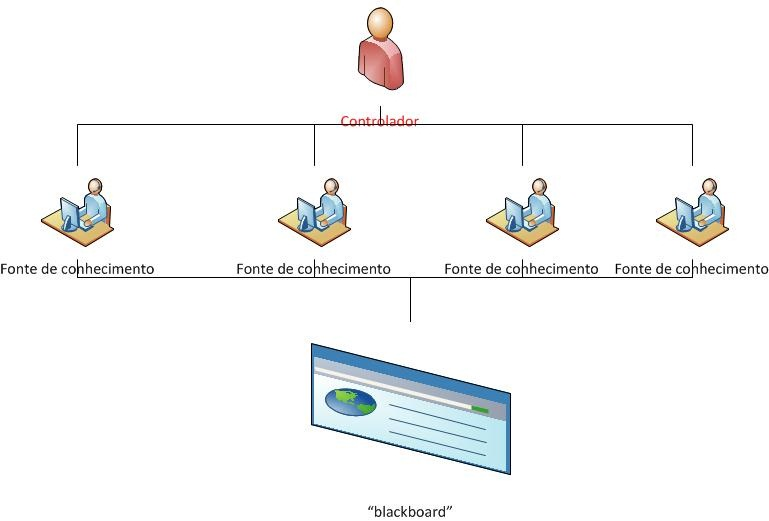
\includegraphics [height=10cm]{figuras/visao_geral_blackboard.jpg}
\caption{Visão geral do blackboard}
\label{blackboard}
\end{figure}
	
Neste projeto utilizaremos a técnica blackboard como parte de um jogo computacional que será desenvolvido.


%Um pouco de história, motivação do uso, desafios e problemas comuns.
\section{Desenvolvimento de jogos}
%Um pouco de como funciona o processo de desenvolvimento de jogos digitias (citar gdd, e empresas!)
A metodologia atual de desenvolvimento de jogos eletrônicos com frequência pode ser dividida nos seguintes passos:
\begin{itemize}
\item Nascimento da idéia: Seja uma pessoa pensando num jogo ou uma equipe inteira fazendo reuniões, o primeiro passo para o desenvolvimento de um jogo é a idéia, nesta etapa é feita uma descrição abstrata do jogo, qual o tipo, os objetivos e desafios que poderão ser criados entre outros.
\item Especificação do documento de game design: O GDD (Game Design Document) é o documento mais importante do processo de desenvolvimento, nele são descritos todos os aspectos do jogo com um alto nível de detalhamento. Uma analogia que existe com a engenharia diz que o GDD é equivalente a uma planta baixa de uma construção, sem ela uma equipe tem todo o material que precisa para construir uma casa mas não sabe por onde começar. O GDD tem o mesmo efeito no processo de desenvolvimento de jogos, as tecnologias necessárias estão presentes, a equipe possui acesso a elas e sabe utilizá-las, porém, sem o GDD, nada fariam.
\item Levantamento dos requisitos de software através do GDD e das decisões de projeto, como por exemplo a plataforma de desenvolvimento que será utilizada gera diversos requisitos.
\item Desenvolvimento, codificação em si e testes.
\end{itemize}

Na lista acima foi ocultada uma etapa comercial do desenvolvimento, em geral o documento de GDD tem uma área de descrição do jogo que é voltada para a propaganda, isto é necessário pois nas grandes empresas, para uma equipe poder desenvolver um jogo é preciso apresentar uma proposta do mesmo para investidores com a finalidade de se conseguir investimentos.


\subsection{Documento de Game Design}
Esta seção apresenta algumas das características principais do documento de design do jogo (GDD). Existem componentes fundamentais em um documento de design completo de um jogo. Esses componentes podem ser documentados separados ou podem ser agrupados em um metadocumento de design do game, que aborda todos os aspectos do design. \cite{design_games}

O documeto de design é criado por uma equipe de design em diversas etapas. Primeiro, o conceito essencial é delineado em um breve documento de visão geral que exlplica os princípios mais importantes do jogo e alguns de seus principais recursos.
Geralmente este documento deve ser aprovado pela empresa que irá desenvolver para que o projeto tenha continuação, uma vez aprovado, começam os trabalhos no documento de design que delineiam todos os aspectos do jogo, incluindo por exemplo, missões, recursos, personagens, níveis, entre outros. Nesta etapa, programadores de scipts já podem iniciar seu trabalho.

A seguir é apresentada a estrutura de um documento completo de design de um jogo extraída de \cite{design_games}

\begin{enumerate}
\item Visão geral essencial
\begin{itemize}
\item Resumo
\item Aspectos fundamentais
\item ``Golden nuggets''
\end{itemize}
\item Contexto do jogo
\begin{itemize}
\item História
\item Eventos anteriores
\item Principais jogadores
\end{itemize}
\item Objetos essenciais do jogo
\begin{itemize}
\item Personagens
\item Armas
\item Estruturas
\item Objetos
\end{itemize}
\item Conflitos e soluções
\item Inteligência Artificial
\item Fluxo do jogo
\item Controles
\item Variações de jogo
\item Definições
\item Referências
\end{enumerate}


A principal função da primeira seção do documento é fazer com que qualquer pessoa se familiarize rapidamente com a idéia do jogo, o que o fará se destacar e --- ter boa jogabilidade.
\subsubsection{Resumo}
O resumo é uma síntese de toda a experiência do jogo.
\subsubsection{Aspectos fundamentais}
O objetivo desta seção é extrair componetes fundamentais do jogo que constituirão a trama central para a experiência e a diversão do jogador.
\subsubsection{Golden Nuggets}
Esta seção deve listar os elementos do jogo que o diferenciam dos concorrentes.

\bigskip

Na segunda seção do documento é definido o contexto do jogo. Todo jogo existe dentro de um contexto que é essencial para se entender o que acontece no mesmo.

\bigskip

\subsubsection{História do jogo}
Nesta seção  história do jogo deve ser explicada desde o seu início até o seu final.
\subsubsection{Eventos anteriores}
Esta seção explica o contexto da história do jogo. Dependendo da simplicidade do projeto pode ser vazia.
\subsubsection{Principais jogadores}
Se no projeto do jogo os personagens forem elementos-chave, nesta seção devem ser apresentados e explicados os principais personagens do jogo.

\bigskip

Na terceira seção do documento são descritos os diversos objetos que aparecem no jogo.

\subsubsection{Personagens}
Esta seção descreve os personagens do jogo, desde os principais personagens envolvidos na histório da jogo aos \npc{}s aliados ou inimigos menos importantes.
\subsubsection{Armas}
Esta seção estabelece quaisquer armas ou habilidades que desempenham papel essencial no jogo.
\subsubsection{Estruturas}
Esta seção define quaisquer estruturas singulares e significativas encontradas no jogo.
\subsubsection{Objetos}
Nesta seção são definidos todos os objetos relevantes que não se encaixam em nenhuma das categorias anteriores.

\bigskip

A quarta seção do documento, ``Conflitos e Soluções'' é normalmente muito detalhada se o combate for um dos principais desafios para o usuário. Todo jogo tem alguma forma de conflito e solução, e essa a área do documento usada para descrevê-los em detalhes.



Na quinta seção, ``Inteligência Artificial'' são resumidos quaisquer comportamentos que definem as ações dos \npc{}s e quaisquer informações (por parte de IA) que afetam esses comportamentos.

\bigskip

A seção ``Fluxo do jogo'', que pode ser uma das mais longas de todo o documento, é basicamente o guia dos programadores, artistas, designers de níveis e de missões. Aqui devem ser detalhados todos os aspectos de como o jogo funcionará.


A seção ``Controles'' do documento abrange os comandos e controles do usuário.

A seção ``Variações de jogo'' abrange qualquer variação prevista no modo de jogar. Se o jogo possuir um único modo de jogar, esta seção torna-se desnecessária.


A seção ``Definições'' só é necessária se na descrição do jogo forem usados alguns termos que não sejam claros.

E finalmente, a seção ``Referências'' contém informações sobre qualquer material de referência que seja essencial para ajudar a captar o clima e a idéia do jogo.


No projeto foi elaborado um documento de design de jogo baseado na estrutura descrita anteriormente.



\section{Avaliação}

\subsubsection{Aspectos humanos} 

Embora o escopo deste trabalho esteja mais próximo de uma avaliação de viabilidade do que de uma análise comparativa de desempenho propriamente dita, vale ressaltar que há espaço, e mesmo a necessidade, de que se estude o impacto da aplicação das técnicas de IA (alvo deste estudo) na experiência de jogo resultante.

Assim, é importante que se tenha em mente que trabalhamos sobre a hipótese de que o campo da inteligência artificial tem a contribuir positivamente na adaptabilidade dos próprios roteiros e trama das histórias que permeiam jogos --- visto que sua aplicação já se dá efetivamente em outros contextos. A expectativa é obter um comportamento mais adaptado ao contexto e enredo em relação que se alcança hoje com máquinas de estado, sem sacrificar o controle que o designer possui.

\subsubsection{Aspectos técnicos e de projeto}

Existe um aumento na complexidade dos diálogos, em razão da necessidade de incorporar mais informações de contexto e variantes no jogo. Isso se traduz na composição de um número maior de derivações em diálogos, já que tanto o jogador quanto os \npc{}s passam a ter opções, e também a necessidade de projeto dos agentes em si.

\subsubsection{Aspectos gerais}

É interessante que se avalie o processo de adaptação das técnicas empregadas ao estudo feito, e se elas podem ser aplicadas a outros domínios. Em particular, o que jogos de diferentes gêneros podem ganhar com o uso da engenharia de software voltada a agentes e de técnicas como por exemplo, blackboard.
%O que o estudo de caso vai avaliar, e como. Decisões de projeto que
%validam o estudo (C++, \emph{data-driven} design, prototipação,
%engenharia de software), isto é, porque o projeto permite extrapolar
%conclusões para jogos na indústria.
